% Chapter 2

\chapter{Marco Teórico} % Main chapter title

\label{Chapter2} 

El objetivo de este capítulo fue revisar los fundamentos de la teoría de los sistemas de comunicaciones móviles, comenzando desde las distribuciones de probabilidad utilizadas para caracterizar los fenómenos más importantes en este ámbito, después se ahondó en las pérdidas en un sistema celular por medio de los modelos de canal más comunes y con su caracterización en parámetros a larga y pequeña escala, p.ej., la pérdida por trayectoria y el desvanecimiento de las señales de radio.\newline

Además, se repasó la teoría del concepto celular, es decir, la geometría celular clásica que sirve para la eficiencia en la planificación de los recursos y por lo tanto el problema más importante en estos sistemas: los efectos de la interferencia. \newline

Finalmente, se revisaron los aspectos de la teoría del tráfico en telecomunicaciones, los organismos más importantes de estandarización de redes móviles y algunos conceptos de las simulaciones a nivel de sistema orientados a eventos discretos en conjunto con los lenguajes de programación más utilizados.\newline


%----------------------------------------------------------------------------------------
%	SECTION 1
%----------------------------------------------------------------------------------------

\section{DISTRIBUCIONES ESTADÍSTICAS EN TELECOMUNICACIONES}

El uso de modelos estadísticos es importante para describir \parencite{Correia2018}:
\begin{itemize}
    \item Llamadas telefónicas y conexiones de datos
    \item Influencia del usuario en el rendimiento de la red
    \item Propagación no guiada en ambientes aleatorios
    \item Movilidad del usuario
\end{itemize}

Comúnmente se utilizan las siguientes distribuciones de probabilidad en telecomunicaciones \parencite{Correia2018}:

\begin{enumerate}
    \item Distribución Uniforme: Es usada para describir la fase de una señal. También, se ha utilizado para simular el despliegue de BSs \parencite{TurjmanSmallCells}.
    \item Distribución Normal (Gaussiana): Es usada para describir fluctuaciones alrededor de un valor medio, p.ej. shadowing. Esta distribución no puede ser usada para describir entidades que no pueden ser negativas.
    \item Distribución Log-Normal: Es usada para describir entidades como la potencia de una señal, amplitudes, principalmente el desvanecimiento lento.
    \item Distribución Rayleigh: Es usada para describir el desvanecimiento rápido-intenso.
    \item Distribución Susuki: Describe conjuntamente el desvanecimiento lento y rápido.
    \item Distribución Rice: Es usada para describir el desvanecimiento rápido - no-intenso.
    \item Distribución Exponencial: Es ampliamente usada para describir la duración de diferentes fenómenos, principalmente asociados con el desvanecimiento de señales y las llamadas telefónicas.
    \item Distribución de Bernoulli: Es usada para describir la ocupación de canales de telecomunicaciones.
    \item Distribución binomial: Es usada para describir llamadas telefónicas.
    \item Distribución de Poisson: Es usada para describir la generación de llamadas telefónicas.
\end{enumerate}

Las PDF y CDF son de suma importancia en el área de las telecomunicaciones ya que ayudan a caracterizar estadísticamente diferentes fenómenos.\newline

\myworries{TODO: incluir procedimientos para generar variables aleatorias a partir de una distribución uniforme}

%----------------------------------------------------------------------------------------
%	SECTION 
%----------------------------------------------------------------------------------------

\section{MODELADO DEL CANAL CELULAR}

Los modelos de propagación por radio se clasifican en modelos a gran escala y a pequeña escala. Los efectos a gran escala generalmente ocurren en el orden de cientos a miles de metros de distancia. Los efectos a pequeña escala se localizan y ocurren temporalmente (en el orden de unos pocos segundos) o espacialmente (en el orden de unos pocos metros). Los parámetros del canal generalmente se dividen en Pérdida por trayectoria (PL), parámetros de gran escala (LSP, como sombreado, dispersión de retardo, dispersión angular, etc.) y parámetros de pequeña escala (como demora, ángulo de llegada y salida, etc.), que reflejan conjuntamente las características de desvanecimiento del canal. El procedimiento de generación de los coeficientes del canal se puede apreciar en la Figura 1. La pérdida de ruta generalmente se expresa en una o dos fórmulas y un conjunto de valores numéricos de parámetros, que reflejan las relaciones con el entorno de transmisión, la distancia y la frecuencia, etc. \newline

\begin{figure}[th]
\centering
\includegraphics[scale=0.8]{Figures/Procedimiento de generación de coeficientes de canal}
\decoRule
\caption[Procedimiento de generación de coeficientes de canal]{Procedimiento de generación de coeficientes de canal, [Fuente: 3GPP TR36.873]}
\label{fig:Procedimiento de generacion de coeficientes de canal}
\end{figure}

El rendimiento a nivel de enlace es un fenómeno de pequeña escala el cual lidia con cambios instantáneos en el canal a través de áreas e instantes de tiempo pequeños donde se considera la potencia recibida como constante, por otra parte, en las simulaciones a nivel de sistema para determinar el rendimiento en general del sistema para un gran número de usuarios esparcidos en una área geográfica es necesario incorporar parámetros de larga escala como el comportamiento estadístico de la interferencia, así como los niveles de señal experimentados por cada usuario a través de largas distancias, ignorando las características transitorias del canal (las de pequeña escala) \parencite{Tranter2003}. En una simulación a nivel de sistema, principalmente se busca la probabilidad de que un usuario en particular alcance un servicio aceptable en el sistema, para esto es necesario contemplar los efectos de los múltiples usuarios para cada enlace individual entre un móvil y la estación base. Por lo tanto en las simulaciones a nivel de sistema se suelen omitir los parámetros a pequeña escala.\newline

\subsection{Relaciones Generales de Propagación}

La pérdida por trayectoria $L_p\ $ se define como \parencite{Correia2018}:

\begin{equation}
L_{p[dB]}=P_{tx[dBm]}+G_{tx[dBi]}-P_{rx\left[dBm\right]}+G_{rx\left[dBi\right]}
\label{eqn:Lp}
\end{equation}

Donde:\newline
\[P_{tx}\to Potencia\ de\ la\ antena\ transmisora\ \] 
\[G_{tx}\to Ganancia\ de\ la\ antena\ transmisora\ \] 
\[P_{rx}\to Potencia\ de\ la\ antena\ receptora\ \ \] 
\[G_{rx}\to Ganancia\ de\ la\ antena\ receptora\ \ \] 

En muchas aplicaciones la ganancia de la antena es referida al dipolo de media longitud de onda:\newline

\begin{equation}
G_{[dBi]} = G_{[dBd]}+{2.15} 
\label{eqn:Gain}
\end{equation}

La Potencia Isotrópica Radiada Efectiva (EIRP) se define como:

\begin{equation}
P_{EIRP[dBm]}=P_{tx\left[dBm\right]}{\ +\ G}_{tx[dBi]}
\label{eqn:EIRP}
\end{equation}

\subsection{Pérdida por trayectoria en el Espacio Libre (FSPL, \textit{Free Space Path Loss})}

El receptor puede recibir una señal atenuada directa (también llamada señal de línea de vista (LoS)) del transmisor. El FSPL se utiliza para predecir la pérdida de trayectoria cuando hay un LoS claro y sin obstrucciones entre el transmisor y el receptor. Se basa en la ley de distancia al cuadrado inverso que establece que la potencia recibida (PRX) decae por un factor de cuadrado de la distancia (d) desde el transmisor.\newline

Se considera a la propagación en el espacio libre como la mínima atenuación que una señal puede sufrir en el medio.\newline

La potencia disponible en la antena receptora ${\ P}_{rx}$ con una propagación en el espacio libre se define como (también conocida como Formula de Friis):\newline

\begin{equation}
P_{rx\left[W\right]}={\left(\frac{{\lambda }_{[m]}}{4\pi d_{[m]}}\right)}^2P_{tx\left[W\right]}G_{tx}G_{rx}  
\label{eqn:Friis}
\end{equation}

ó\newline

\begin{equation}
P_{rx\left[dBW\right]}=-32.44+P_{tx\left[dBW\right]}+G_{tx\left[dBi\right]}+G_{rx\left[dBi\right]}-20{\mathrm{log} \left(d_{\left[km\right]}\right)\ }-20{\mathrm{log} \left(f_{\left[MHz\right]}\right)\ }
\label{eqn:Friss_dB}
\end{equation}

Donde:\newline
\[d\to Distancia\ entre\ Rx\ y\ Tx\ \] 
\[f\to Frecuencia\ de\ operaci\textrm{\'{o}}n\ \] 
\[\lambda \to Longitud\ de\ onda,\ \ \ \ \ \ \ \ \lambda =\frac{c}{f}\ \] 
\[c\to Velocidad\ de\ la\ luz\ (\mathrm{299\ 792\ 458\ m/s})\] 

Por lo tanto, la p\'{e}rdida por trayectoria en el espacio libre $L_0$ se define como:\newline

\begin{equation}
L_{0[dB]}=32.44+20{\mathrm{log} \left(d_{\left[km\right]}\right)\ }+20\mathrm{log}\mathrm{}(f_{[MHz]})
\label{eqn:Lp}
\end{equation}

Tomando el modelo del decaimiento de potencia promedio con la distancia $a_{pd}$:\newline
\begin{equation}
L_{p[dB]}=L_{ref}+10a_{pd}{\mathrm{log} \left(d_{\left[km\right]}\right)\ }
\label{eqn:Lp_ref}
\end{equation}

\[a_{pd}=2,\ \ \ para\ una\ propagacion\ en\ el\ espacio\ libre\ \] 

El \textit{apd (también conocido como PLE)} es un valor que va de 2 a 4 frecuentemente. El valor mínimo (i.e. 2) proviene de la perdida FSPL y el máximo (i.e. 4) por la pérdida del modelo \textit{Flat Earth} (modelo de tierra plana). En algunos modelos se llega a incluir valores de PLE m\'{a}s altos que los aqu\'{i} definidos.\newline

\subsection{Caracterización del canal de radio}

Usualmente en ambientes urbanos no hay línea de vista (LoS) entre la estación base (BS) y la terminal móvil (MT\footnote{MT y UE son términos análogos.}) [véase Figura~\ref{fig:Propagacion}] por lo que la transmisión es realizada por reflexión, difracción y dispersión de las señales.\newline

\begin{figure}[th]
\centering
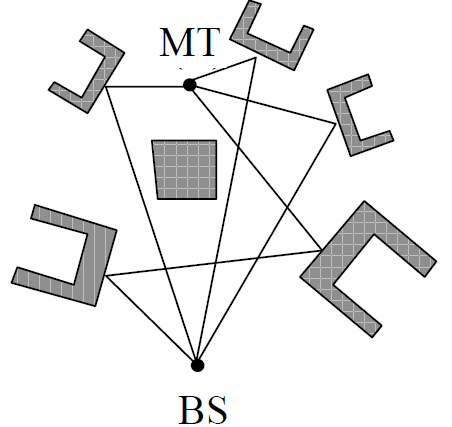
\includegraphics[scale=.5]{Figures/Propagación de señales celulares en ambientes urbanos.}
\decoRule
\caption[Propagación de señales celulares en ambientes urbanos]{Propagación de señales celulares en ambientes urbanos, [Fuente: L. Correia 2018]}
\label{fig:Propagacion}
\end{figure}

Sin embargo estas señales sufren de desvanecimiento con caídas de potencia. Este desvanecimiento depende de la posición y el ambiente del cual se propague la señal.\newline
Características de desvanecimiento:\newline

\begin{itemize}
    \item Desvanecimiento lento:
    Depende esencialmente de la distancia, sigue una distribución Log-normal
    \item Desvanecimiento rápido:
    Es asociado al movimiento del usuario, sigue una distribución Rice
\end{itemize}

\begin{figure}[th]
\centering
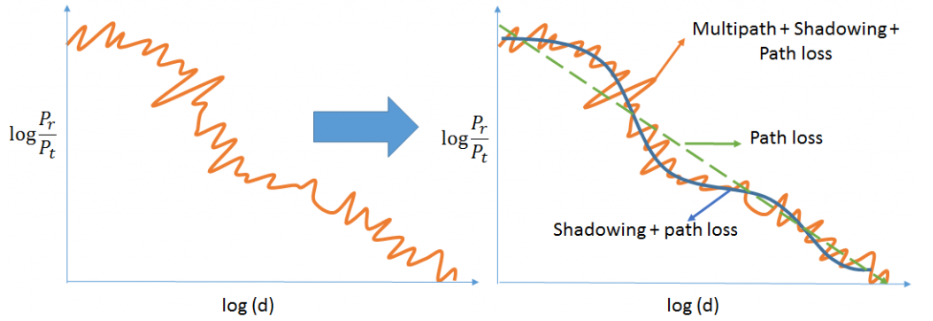
\includegraphics[scale=.5]{Figures/Ejemplo de niveles de señal con desvanecimiento lento y desvanecimiento rápido}
\decoRule
\caption[Ejemplo de niveles de señal con desvanecimiento lento y desvanecimiento rápido]{Ejemplo de niveles de señal con desvanecimiento lento y desvanecimiento rápido, [Fuente: V. Mathuranathan, 2016]}
\label{fig:Desvanecimientos}
\end{figure}

En la Figura~\ref{fig:Desvanecimientos} se observa que al principio, la señal parece muy aleatoria. Mirando más de cerca podemos dividirlo en tres componentes principales como se muestra en la mitad derecha de la Figura~\ref{fig:Desvanecimientos} \parencite{Mathuranathan2016}.\newline

El desvanecimiento lento puede ser causado por eventos como el \textit{shadowing}, donde una gran obstrucción, como una colina o un gran edificio, oscurece la trayectoria de la señal principal entre el transmisor y el receptor. Se considera un parámetro a gran escala.\newline

El desvanecimiento rápido ocurre cuando la amplitud y el cambio de fase impuestos por el canal varían considerablemente durante el período de uso. Una señal que viaja en un entorno puede verse reflejada por varios objetos en el camino. Esto da lugar a varias señales reflejadas. Las señales reflejadas llegan al receptor en diferentes instantes de tiempo y con diferentes intensidades que conducen a la propagación multitrayectoria. Se considera un parámetro a pequeña escala.\newline

Los márgenes de desvanecimiento deben tomarse en cuenta para caracterizar la variación de las señales alrededor de un valor promedio, esto depende de:\newline
•	Características del ambiente (LoS)\newline
•	QoS\newline

Para \textit{narrowband} (banda estrecha, donde prevalece el desvanecimiento plano en lugar de un desvanecimiento selectivo de frecuencia) el desvanecimiento se caracteriza de la siguiente manera:
\begin{itemize}
    \item Desvanecimiento rápido:
    \begin{itemize}
        \item LoS: Distribución Rice (no intenso)
        \item NLoS: Distribución Rayleigh (intenso)
    \end{itemize}
    \item Desvanecimiento lento:
    \begin{itemize}
        \item Distribución Log-Normal
    \end{itemize}
    \item Ambos desvanecimiento rápido y lento:
    \begin{itemize}
        \item Distribución Susuki
    \end{itemize}
\end{itemize}

Los modelos de estimación de señal pueden ser divididos en dos categorías:
\begin{enumerate}
    \item Teóricos:Son una aproximación a la realidad, no toman en cuenta todos los factores de la propagación pero permiten cambios fáciles de los parámetros. 
    \begin{itemize}
        \item Ray Tracing
        \item Modelo Ikegami [1984]
        \item Modelo Walfish-Bertoni [1988]
    \end{itemize}
    \item Empíricos: Están basados en la observación de mediciones, conduciendo al mejor ajuste de ecuaciones. Tienen la ventaja de tomar en cuenta todos los factores que influyen en la propagación.\newline
    Para ambientes exteriores hay dos modelos básicos:\newline
    \begin{itemize}
        \item COST 231 Okumura-Hata
        \begin{itemize}
            \item Largas distancias (>5km)
            \item Ambientes rurales, urbanos y suburbanos
            \item Alta desviacion estandar
            \item Rango de frecuencias aplicables [1.5,2.0] GHz
        \end{itemize}
        \item COST 231 Walfish-Ikegami [1999]
        \begin{itemize}
            \item Cortas distancias (<5km)
            \item Ambientes urbanos y suburbanos
            \item Rango de frecuencias aplicables [.8,2.0] GHz
        \end{itemize}
        \item COST 207 [1989]
    \end{itemize}
\end{enumerate}

%----------------------------------------------------------------------------------------
%	SECTION 
%----------------------------------------------------------------------------------------

\section{GEOMETRÍA CLÁSICA CELULAR}
\subsection{Planeación Celular}
\subsection{Planeación de frecuencia}

%----------------------------------------------------------------------------------------
%	SECTION 
%----------------------------------------------------------------------------------------

\section{INTERFERENCIA EN SISTEMAS CELULARES}

%----------------------------------------------------------------------------------------
%	SECTION 
%----------------------------------------------------------------------------------------

\section{CAPACIDAD EN SISTEMAS DE COMUNICACIONES}

%----------------------------------------------------------------------------------------
%	SECTION 
%----------------------------------------------------------------------------------------

\section{INTERFAZ DE RADIO}
\subsection{Esquemas de Acceso Múltiple al Medio}
\subsection{Generaciones anteriores de sistemas de comunicaciones móviles}

%----------------------------------------------------------------------------------------
%	SECTION 
%----------------------------------------------------------------------------------------

\section{TELETRÁFICO}
\subsection{Caracterización del Tráfico}
\subsection{Notación Kendall}

%----------------------------------------------------------------------------------------
%	SECTION 
%----------------------------------------------------------------------------------------

\section{SIMULACIONES ORIENTADAS A EVENTOS DISCRETOS}

%----------------------------------------------------------------------------------------
%	SECTION 
%----------------------------------------------------------------------------------------

\section{SIMULACIÓNES A NIVEL DE SISTEMA}

%----------------------------------------------------------------------------------------
%	SECTION 
%----------------------------------------------------------------------------------------

\section{LENGUAJES DE PROGRAMACIÓN PARA SIMULACIONES ORIENTADAS A EVENTOS DISCRETOS (DES)}
\subsection{Python}
\subsection{Librería Simpy}
%----------------------------------------------------------------------------------------
%	SECTION 
%----------------------------------------------------------------------------------------

\section{ORGANISMOS INTERNACIONALES DE ESTANDARIZACIÓN}
